% Preamble

\documentclass[12pt,a4paper]{article}
\usepackage[top=25mm, bottom=25mm, left=25mm, right=25mm]{geometry}
%\usepackage[document]{ragged2e}   % left-justified (or flush-left) rather than fully-justified for the entire document

\usepackage{setspace}    % for line spacing
\renewcommand{\baselinestretch}{1.2}
\parskip = \medskipamount
\parindent = 0pt   % This will remove the paragraph indent
\frenchspacing

\usepackage{xcolor}
\definecolor{darkblue}{rgb}{0,0,0.3}
\definecolor{codegreen}{rgb}{0,0.6,0}
\definecolor{codegray}{rgb}{0.5,0.5,0.5}
\definecolor{codepurple}{rgb}{0.58,0,0.82}
\definecolor{backcolour}{rgb}{0.95,0.95,0.92}
\definecolor{light-gray}{gray}{0.95}
\newcommand{\code}[1]{\colorbox{light-gray}{\texttt{#1}}}

\usepackage[english]{babel}
\usepackage{epsfig}
\usepackage[utf8]{inputenc}
\usepackage{tabularx}
\usepackage{longtable}
\usepackage{booktabs}
\usepackage{microtype}   % for micro-typographical adjustments
\usepackage{enumitem}
\usepackage{amsmath,amssymb,amsfonts}
\usepackage{pifont}
\usepackage{siunitx}   %  SI units package (http://mirrors.ibiblio.org/CTAN/macros/latex/contrib/siunitx/siunitx.pdf)
\usepackage{framed}
\usepackage{footnote}
\usepackage{caption}
\usepackage{subcaption}
\usepackage{hyphsubst}
\usepackage[none]{hyphenat} 
\usepackage[autostyle]{csquotes}
\usepackage{listings}
\usepackage{times}
\usepackage{a4wide}
\usepackage{textcomp}

\usepackage{graphicx}
\usepackage{float}
\graphicspath{ {./images/} }

\usepackage{tocloft}
\renewcommand{\cftsecleader}{\cftdotfill{\cftdotsep}}
\setlength\cftparskip{-0.5pt}

\usepackage{tikz}
\def\checkmark{\tikz\fill[scale=0.4](0,.35) -- (.25,0) -- (1,.7) -- (.25,.15) -- cycle;}

\usepackage{fancyhdr}
\pagestyle{fancy}
% \pagestyle{plain}   % This is the default style. The header is empty and the footer contains page numbers in the centre.
% \pagestyle{empty}   % Both the header and footer are cleared (blank).
\fancyhf{}   % clears the header and footer, otherwise the elements of the default "plain" page style will appear.
\fancyhead{}
\fancyfoot{}
\fancyhead[L]{Parallelization of a Sudoku Solver}
\fancyhead[R]{Hua-Ming Huang}   % Options: \leftmatk, \rightmark, \thepage, \thesection, \thechapter, etc.
\usepackage{lastpage}
\fancyfoot[C]{\thepage\ / \pageref*{LastPage}}
% \fancyfoot[R]{Page \thepage \hspace{1pt} of \pageref{LastPage}}
% Decorative lines on header and footer
\renewcommand{\headrulewidth}{0.4pt}
\renewcommand{\footrulewidth}{0.4pt}   % Default: 0pt thickness. Hence is not visible

\usepackage{biblatex}
\addbibresource{references.bib}

% hyperref should be the last package you load
\usepackage{hyperref}
\hypersetup{
	colorlinks=true,
	linkcolor=codegreen,
	citecolor=blue,
	filecolor=codegray,
	urlcolor=darkblue
}

\lstdefinestyle{pyt}{
    backgroundcolor=\color{backcolour},   
    commentstyle=\color{codegreen},
    keywordstyle=\color{magenta},
    numberstyle=\tiny\color{codegray},
    stringstyle=\color{codepurple},
    basicstyle=\ttfamily\footnotesize,
    breakatwhitespace=false,         
    breaklines=true,                                    
    keepspaces=true,                 
    numbers=left,                    
    numbersep=5pt,                  
    showspaces=false,                
    showstringspaces=false,
    showtabs=false,                  
    tabsize=4
}

\lstset{style=pyt}

\newcommand{\horrule}[1]{\rule{\linewidth}{#1}}

% ------------------------ End of Preamble ------------------------
\begin{document}
\sloppy


\begin{titlepage}
% Declare new goemetry for the title page only
\newgeometry{left=25mm, right=25mm, top=25mm, bottom=25mm}
\begin{figure}[H]
	\centering
	
\includegraphics[height=20mm]{tum.pdf}
\end{figure}
\begin{center}
	\large
    \textbf{1 ECTS Study Project of the Module Parallel Computing (BV440004) SS21\textquotesingle}\\[10pt]
    \normalsize
	\textsc{Chair of Computational Modeling and Simulation}\\
	\textsc{Department of Civil, Geo and Environmental Engineering}\\
	\textsc{Technical University of Munich}\\
	Arcisstraße 21\\
	D-80333 München\\ 
    \vfill
    \LARGE
	\horrule{1.5pt}\\[0.4cm]
    \textbf{Parallelization of a Sudoku Solver}\\
    \Large
    \vspace{.25cm}
    - Project Report -\\
	\horrule{1.5pt}\\[0.4cm]
    \vfill
	\begin{figure}[H]
		\centering
		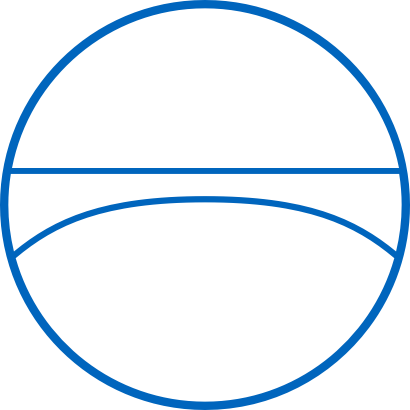
\includegraphics[height=15mm]{TUM_BGU_logo}
	\end{figure}
    \large
    Hua-Ming Huang\\
	\href{mailto:huaming.huang.tw@gmail.com}{huaming.huang.tw@gmail.com}\\
    \vfill
    \normalsize
    \begin{tabular*}{\textwidth}{l @{\extracolsep{\fill}} r}    
    \toprule
    \textbf{\textit{Supervisor:}}  & Christoph Ertl\\
    \bottomrule
    \end{tabular*}
    \thispagestyle{empty}
\end{center}
\end{titlepage}


% Ends the declared geometry for the title page
\restoregeometry


\newpage %%%%%%%%%%%%%%%%%%%%%%%%%%%%%%%%%%%%%%%%
{\hypersetup{linkcolor=black}
\begin{spacing}{2.0}
    \clearpage
    \tableofcontents
    \thispagestyle{empty}
    \setcounter{page}{0}
\end{spacing}
}


\newpage %%%%%%%%%%%%%%%%%%%%%%%%%%%%%%%%%%%%%%%%
\section{Introduction}

	\subsection{What is Sudoku?}
	A Sudoku puzzle is a $n$-by-$n$ grid that contains numbers from \num{1} to $n$, with box size $\sqrt{n} \times \sqrt{n}$.
	A standard Sudoku contains \num{81} cells, in a \numproduct{9 x 9} grid, and has \num{9} boxes (\numproduct{3 x 3} grid),
	as shown in Figure \ref{fig:standard-Sudoku-puzzle}.

	\begin{figure}[H]
		\centering
		\begin{subfigure}{.5\textwidth}
			\centering
			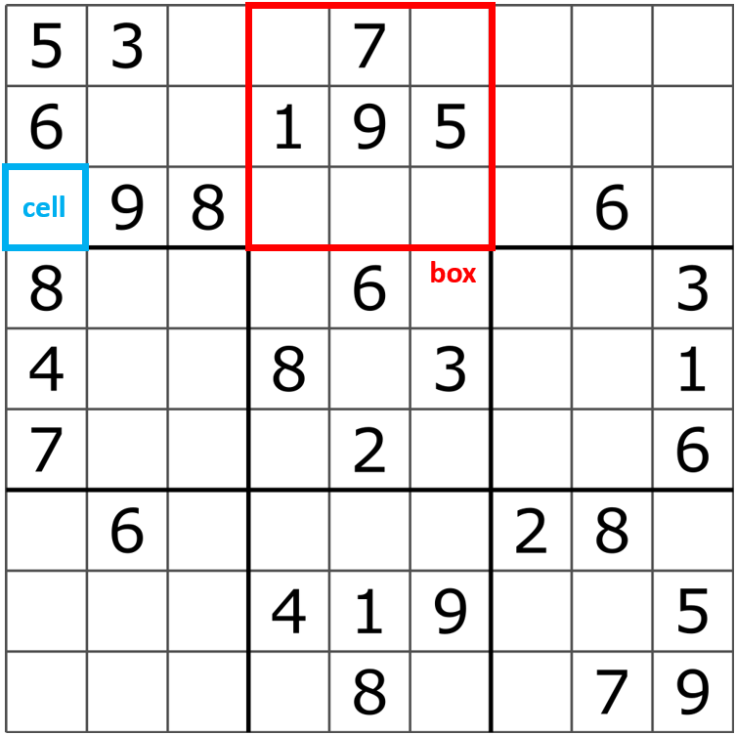
\includegraphics[height=0.8\linewidth]{9x9_puzzle}
		\end{subfigure}%
		\begin{subfigure}{.5\textwidth}
			\centering
			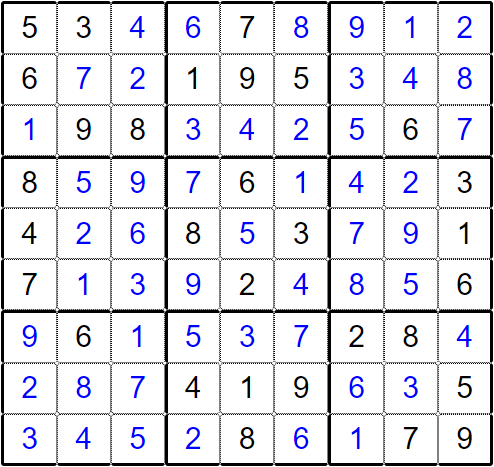
\includegraphics[height=0.8\linewidth]{9x9_solution}
		\end{subfigure}
		\caption{A typical Sudoku puzzle (\textsl{left}) and its solution (\textsl{right})}
		\label{fig:standard-Sudoku-puzzle}
	\end{figure}

	The goal of the puzzle game is to fill in the empty cells on the board such that each column,
	row, and box (or called ``subgrid'', ``region'', ``block'') contains every number in the set $\{1, ... , 9\}$ exactly once.
	Sudoku puzzles usually come with a partially filled-in board (\textit{clues}).
	The difficulty of the puzzle varies depending on how many numbers are given, as well as the location of the given numbers.
	There are many strategies to solve Sudoku puzzles (See Section \nameref{sec:solving-algorithms}).
	Solutions might not be unique, or might not even exist.
	However, a properly formulated Sudoku puzzle should have an unique solution that can be reached logically.
	
	\subsection{Rules of Sudoku} \label{sec:rules}
	\begin{itemize}[itemsep=0pt, parsep=0pt]
		\item Each number must appear exactly once in each row.
		\item Each number must appear exactly once in each column.
		\item Each number must appear exactly once in each box.
	\end{itemize}
	
	The above rules imply no \textit{duplicate} numbers in any row, column and box.


\newpage %%%%%%%%%%%%%%%%%%%%%%%%%%%%%%%%%%%%%%%%
\section{Motivation}
Thanks to the computational power provided by modern computers, there are already several algorithms (See Section \nameref{sec:solving-algorithms})
that will solve \numproduct{9 x 9} Sudoku puzzles in fractions of a second.
However, as the size of Sudoku puzzle $n$ gets larger, e.g.,
\numproduct{16 x 16}, \numproduct{25 x 25} (Figure \ref{fig:large-Sudoku-puzzles}),
the \textit{combinatorial explosion} occurs and thus leads to \textit{exponential} growth of overall solving time.
Combinatorial explosion creates limits to the properties of Sudokus that can be constructed, analyzed, and solved \cite{wiki:combinatorial-exploration}. 
This also directly eliminates the possibility of solving Sudoku in a reasonable amount of time.

\begin{figure}[H]
	\centering
	\begin{subfigure}{.5\textwidth}
		\centering
		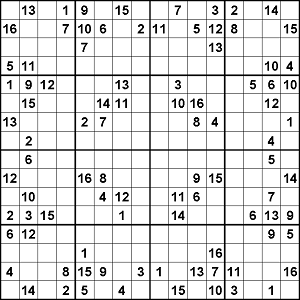
\includegraphics[height=0.95\linewidth]{16x16_puzzle}
		\caption{A \numproduct{16 x 16} Sudoku puzzle}
		\label{fig:sub1}
	\end{subfigure}%
	\begin{subfigure}{.5\textwidth}
		\centering
		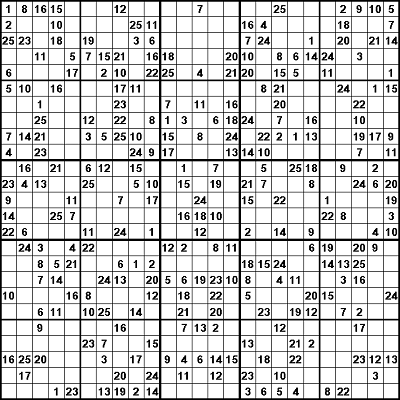
\includegraphics[height=0.95\linewidth]{25x25_puzzle}
		\caption{A \numproduct{25 x 25} Sudoku puzzle}
		\label{fig:sub2}
	\end{subfigure}
	\caption{Large Sudoku puzzles}
	\label{fig:large-Sudoku-puzzles}
\end{figure}

Therefore, this project aims to implement a Sudoku solver that could solve \textbf{large} Sudoku puzzles
as efficiently as possible by means of various parallelization techniques and algorithms.


\newpage %%%%%%%%%%%%%%%%%%%%%%%%%%%%%%%%%%%%%%%%
\section{Solving Algorithms} \label{sec:solving-algorithms}
	\cite{wiki:Sudoku-solving-algorithms}

	\subsection{Naive brute-force algorithm} \label{sec:brute-force-algorithms}
	A brute-force algorithm would enumerate \textit{all} possible combinations of numbers for each empty cell.
	This algorithm has an incredibly large search space to wade through.
	For instance, a blank $n$-by-$n$ grid has a total of $n^{n \times n}$ different possible combinations of solutions.
	Solving Sudoku puzzles in this way is extremely slow and computationally intensive,
	but guarantees to find a solution eventually and the solving time is mostly unrelated to degree of difficulty.

	\subsection{Backtracking algorithm}
	A common algorithm to solve Sudoku boards is called \textit{backtracking},
	which is a type of brute-force search.
	This algorithm is essentially a \textit{depth-first search (DFS)} by completely exploring one
	branch to a possible solution before moving to another branch.
	
	Given a partially filled-in (incomplete) board, the following illustrates the backtracking algorithm
	step by step: \cite{techwithtim:backtracking}

	\begin{enumerate}
		\item Finds the first empty cell on the given board.
		\item Attempts to place the smallest possible number (namely \num{1}) in that cell.
		\item Checks if the inserted number is valid.
			\begin{itemize}
				\item If the number is valid (i.e., does not violate the rules stated in Section \nameref{sec:rules}),
				proceed to the next empty cell and \textbf{recursively} repeat steps \num{1}-\num{3}.
				\item If the number is not valid, increment its number by \num{1} and repeat step \num{3}. If a cell is
				discovered where none of the possible numbers is allowed, then reset the cell you just
				filled to zero/blank and backtrack to the most recently filled cell. The value in that
				cell is then incremented by \num{1} and repeat step \num{3}.
				If the number still cannot be incremented, then we backtrack again.
			\end{itemize}
		\item Repeats the procedure until either there are no more empty cells on the board, which means
		we have found the solution. Or we backtracked to the first unfilled cell. In this case, no
		solution exists for the given board.
	\end{enumerate}

	Rather than trying to continue a solution that can never possibly work which we do with naive
	brute-force algorithm, we \textit{only} continue solutions that currently work.
	If they don’t work, we backtrack to the previous step and try other numbers again.
	This is going to be much faster than trying every single possible combination of solutions
	as naive brute-force algorithm does.

	\subsection{Dancing Links algorithm}
	The Dancing Links algorithm developed by Dr. Donald Knuth is an algorithm for solving the \textit{exact cover problem},
	where some constraints need to be applied. The exact cover problem can be represented by a matrix of \num{0}s and \num{1}s and
	the Dancing Links algorithm will find a set of rows such that the number \num{1} appears in each column exactly once.
	\cite{knuth2000dancing}\cite{java-dancing-links}\cite{wiki:DLX} 
	
	As Sudoku is a special case of the exact cover problem, we can model a Sudoku puzzle in the form of a (sparse) cover matrix:
	\begin{itemize}
		\item The \textit{columns} of cover matrix represent the \num{4} constraints of the Sudoku puzzle:
		\begin{itemize}
			\item \textbf{Cell constraint:} Each cell contains only an integer between \num{1} and $n$ which corresponds to the size of the baord.
			\item \textbf{Row constraint:} Each row contains numbers in the set $\{1, ... , n\}$ exactly once.
			\item \textbf{Column constraint:} Each column contains numbers in the set $\{1, ... , n\}$ exactly once.
			\item \textbf{Box constraint:} Each box contains numbers in the set $\{1, ... , n\}$ exactly once.
		\end{itemize}
		Each number comes with its own set of constraints. Therefore, there are \textbf{$n \times n \times 4$} columns.
		\item The \textit{rows} of cover matrix represent every single possible position for every number.
		Therefore, there are \textbf{$n \times n \times n$} rows.
	\end{itemize}

	The initial state of the board can be expressed by selecting which rows are in the exact coverage.
	The Dancing Links algorithm will then give us a subset of rows where each constraint is filled exactly once and thus the solution to the Sudoku board.


\newpage %%%%%%%%%%%%%%%%%%%%%%%%%%%%%%%%%%%%%%%%
\section{Implementation Details \& Performance Results}
	Please accomany this section with the code and comments in the corresponding \code{*.hpp} and \code{*.cpp} files.
	Only some key aspects will be listed below.

	\subsection{Sequential backtracking algorithm}
		\begin{itemize}
			\item A backtracking algorithm visits the empty cells in some order, filling in possible digits sequentially, or backtracking when the number is found to be not valid. \cite{wiki:Sudoku-solving-algorithms}
			\item There are no parallelizations done for this algorithm because of the following reasons:
				\begin{itemize}
					\item Since backtracking is a depth-first search (DFS), it is not directly parallelizable - because this algorithm depends on the \textit{stack},
					which is implicit in the function call stack. Stacks are hard to parallelize because threads cannot all work on the same stack and efficiently move forward in the algorithm together
					without causing very high contention for accessing to the stack. Therefore, any newly computed result cannot be directly used by another thread.
					\item With the \code{boolean} return type of backtracking algorithm (since the recursion \textit{only} continues solutions that currently work,
					a \code{boolean} checking is required), it's also hard to parallelize. Instead, functions with \code{void} return type is much easier to parallelize.
				\end{itemize}
		\end{itemize}

	\subsection{Sequential brute-force algorithm}
		As stated in \ref{sec:brute-force-algorithms}, brute-force algorithm is guaranteed to find a solution since it tries every possible number in each empty cell.
		This algorithm is very effective for \numproduct{9 x 9} puzzles. Unfortunately for \numproduct{16 x 16} (or \numproduct{25 x 25}) puzzles
		there are \num{16} (or \num{25}) possibilities for each empty cell. This means that there are roughly $16^{16^{2} - n}$ (or $25^{25^{2} - n}$)
		possible states that might need to be searched, where $n$ is the number of filled-in cells in the given Sudoku puzzle.
		It turns out that the brute-force algorithm scales very badly (Figure \ref{fig:sequential-brute-force}).
		\begin{figure}[H]
			\centering
			\frame{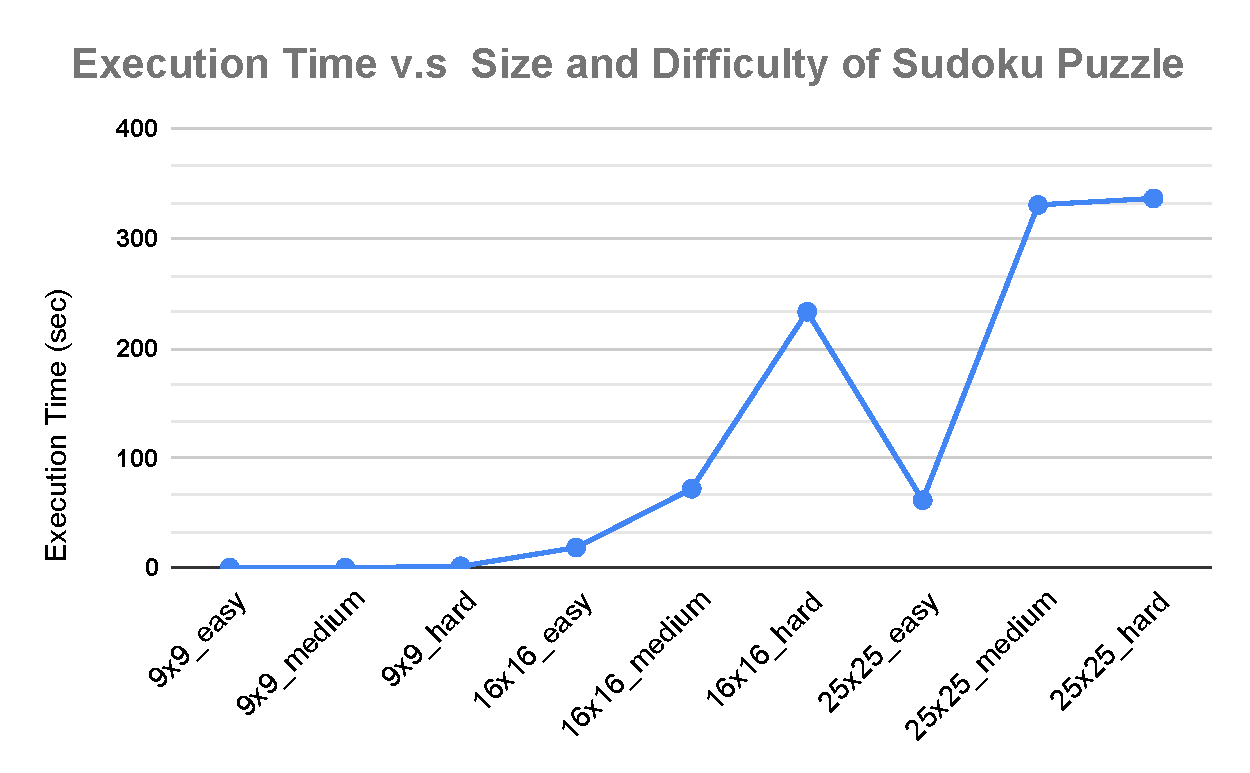
\includegraphics[width=0.7\linewidth]{sequential_brute_force}}
			\caption{}
			\label{fig:sequential-brute-force}
		\end{figure}

	\subsection{Parallel brute-force algorithm}
		There are 3 versions of this implementation:\\
		\code{solve\_bruteforce\_par}, \code{solve\_kernel\_1} and \code{solve\_kernel\_2}
		
		\begin{itemize}[itemsep=0pt, parsep=0pt]
			\item \code{solve\_bruteforce\_par}: Exploit OpenMP tasks for parallelism on multiple recursion levels and
			prevent overhead of task creation by setting a threshold for the recursion depth.
			If the recursion depth is larger than the threshold, switch to \code{solve\_bruteforce\_seq}.
			\item The ideas of \code{solve\_kernel\_1} and \code{solve\_kernel\_2} are the same: Similar to backtracking algorithm, brute-force algorithm is also a depth-first search (DFS) and doesn't appear to be very parallelizable.
			In contrast, breadth-first search (BFS) is easy to parallelize. So we can modify the depth-first search (DFS) approach such that threads can work independently without reading from the same stack.
			Namely, we can parallelize over different branches of the depth-first search (DFS). This approach is summarized as follows:
			\begin{enumerate}[itemsep=0pt, parsep=0pt]
				\item Pushes the input board onto the board deque to initialize a list of incomplete (or intermediate) solutions.
				(The deque scheme for parallization is inspired by this GitHub repo: \cite{github:chr1shr})
				\item \textbf{Bootstrapping}
					\begin{enumerate}[itemsep=0pt, parsep=0pt] 	
						\item Pops a new Sudoku board from the front of the board deque.
						\item Serially fills in empty cells with all possible numbers on this board, and pushes the newly created grids into the deque accordingly.
						This step expands the search tree in a BFS manner. Whenever an empty cell has no possible numbers, prune the DFS tree, i.e., ignore the branch.
						\item Repeats step (a) and (b) till the specified level of bootstrapping is reached.
						This may give us something like thousands of possible boards on the deque to be solved by each thread. 
						An example of bootstrapping to level \num{5} with \code{Test\_Cases/9x9\_easy.txt} as input grid is illustrated in Figure \ref{fig:bootstrapping}.
						\begin{figure}[H]
							\centering
							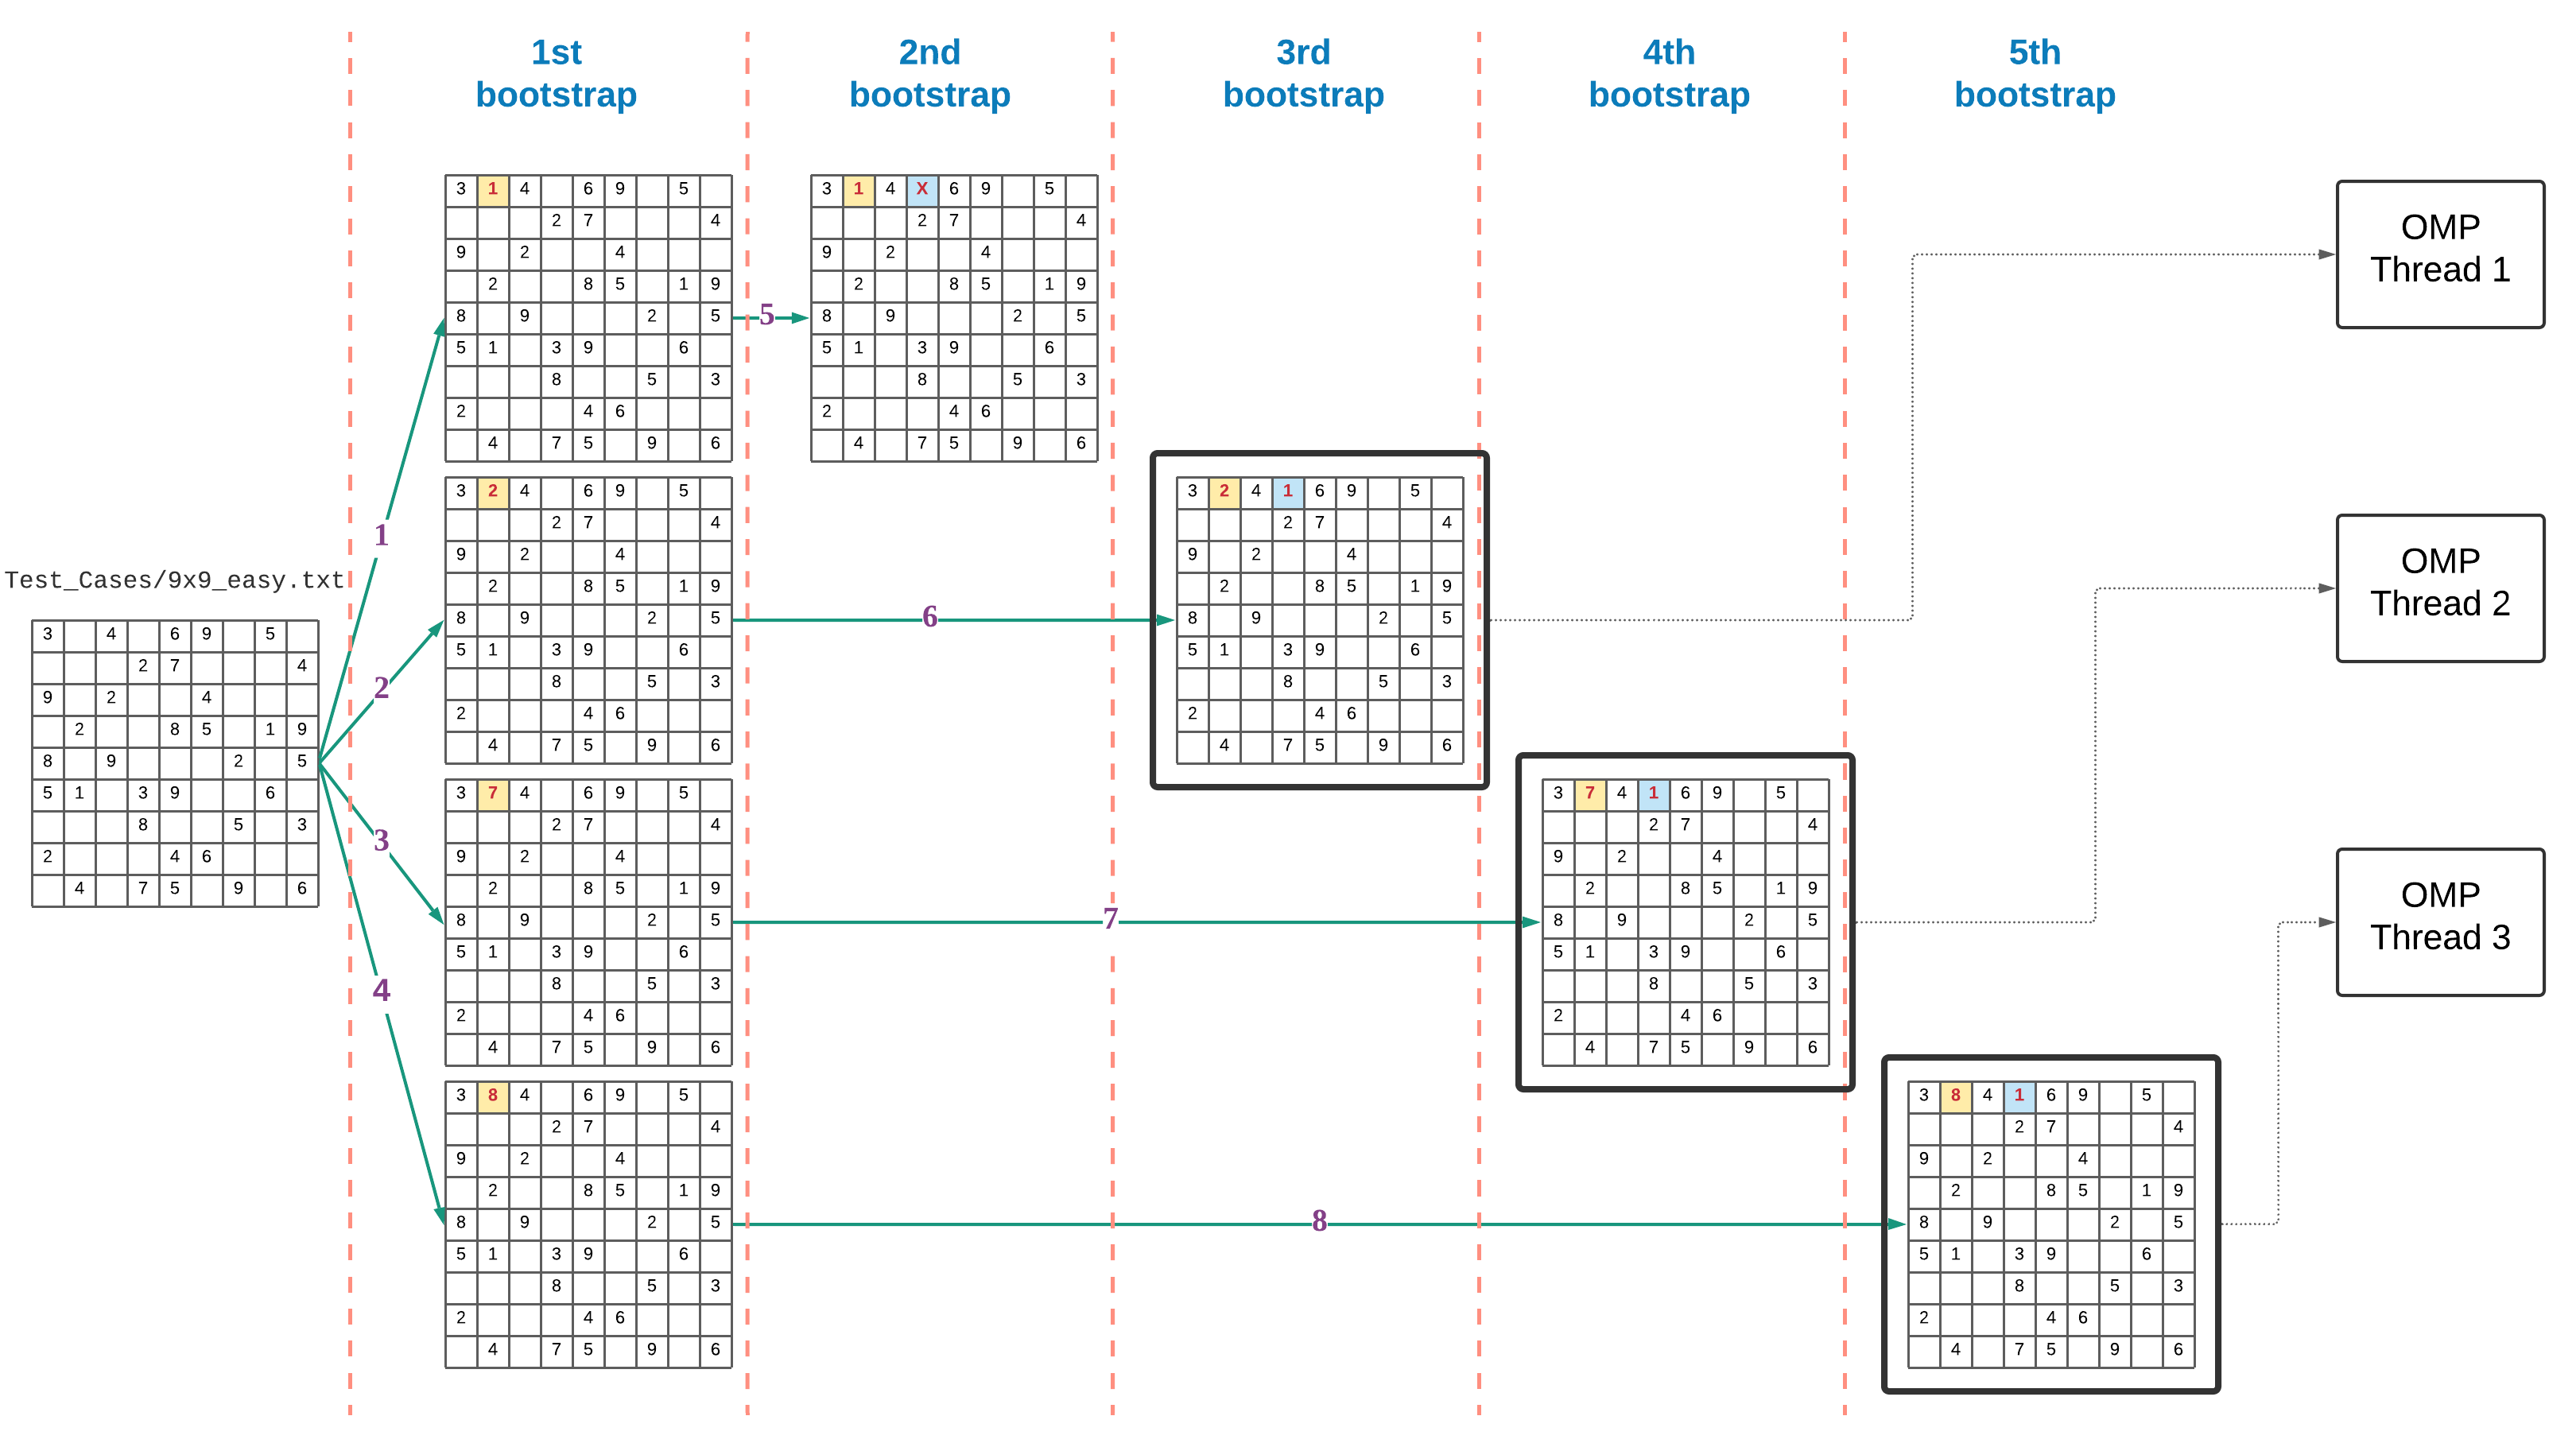
\includegraphics[width=\linewidth]{Bootstrapping}
							\caption{}
							\label{fig:bootstrapping}
						\end{figure}
					\end{enumerate}
				\item Each OpenMP thread gets a Sudoku board from the board deque as starting points respectively and applies sequential brute-force solving algorithm (DFS) on its own board in parallel.
				(Use static scheduling to balance the workload among all threads in round-robin fashion because each thread solves exactly one board.)
				\item Whenever the solution is found in one of the spawned threads, a flag variable is set to \code{true} and the remaining iterations will be skipped by the \code{continue} statement.
			\end{enumerate}
			
			\ding{104} \textbf{Discussion:} As seen from the performance result in Figure \ref{fig:parallel-brute-force}, this competitive parallelization approach is not scalable with respect to the number of OMP threads,
			which is set equal to the level of bootstrapping in the current version of implementation.
			I found the main overhead of this parallelization approach comes from the \textit{level of bootstrapping}, whcih is critical and should be obtained by some optimization metrics.
			If a non-optimal value of bootstrapping level is chosen, the limitation of scalibility will be created and no visible speed-up will be measured.
			\begin{figure}[H]
				\centering
				\frame{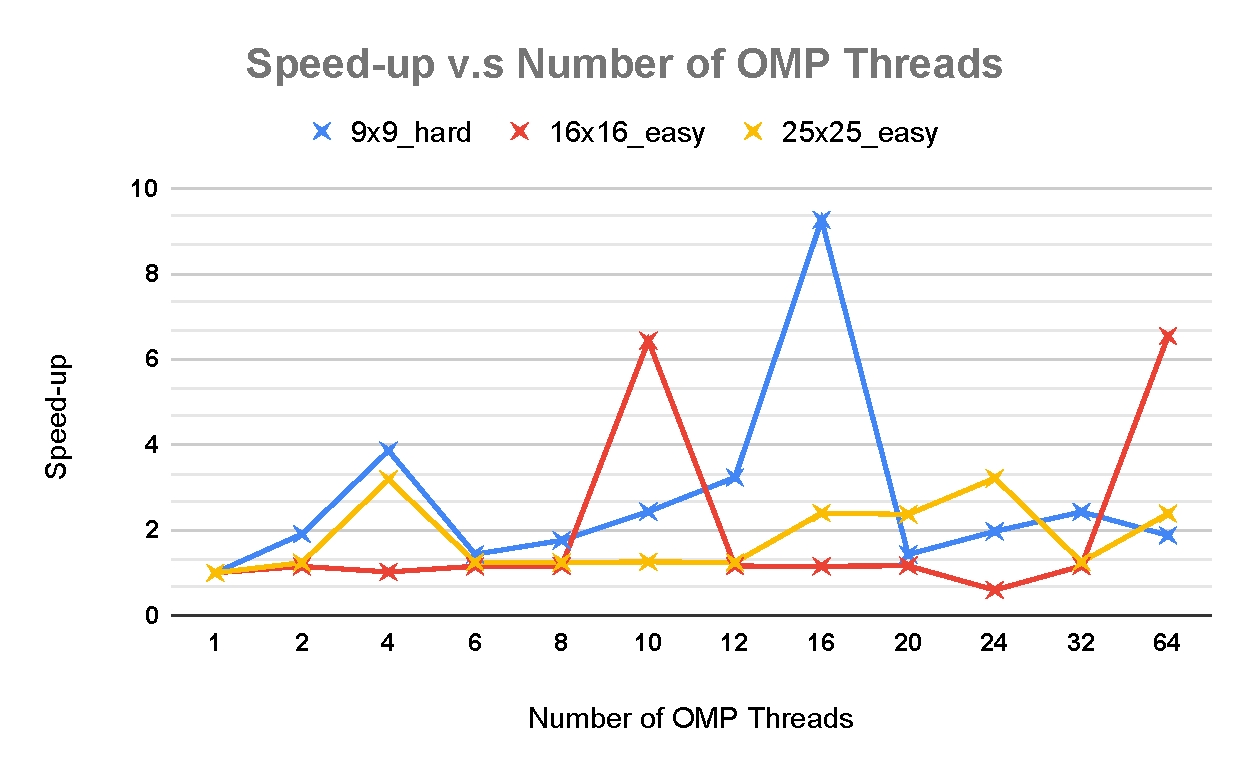
\includegraphics[width=0.7\linewidth]{parallel_brute_force}}
				\caption{}
				\label{fig:parallel-brute-force}
			\end{figure}
		\end{itemize}

	\subsection{Sequential DLX algorithm}
		With the Dancing Links algorithm, even complex Sudoku puzzles can be solved
		very quickly and efficiently as indicated in Figure \ref{fig:sequential-dlx}.
		This performance result can be compared to Figure \ref{fig:sequential-brute-force}.
		\begin{figure}[H]
			\centering
			\frame{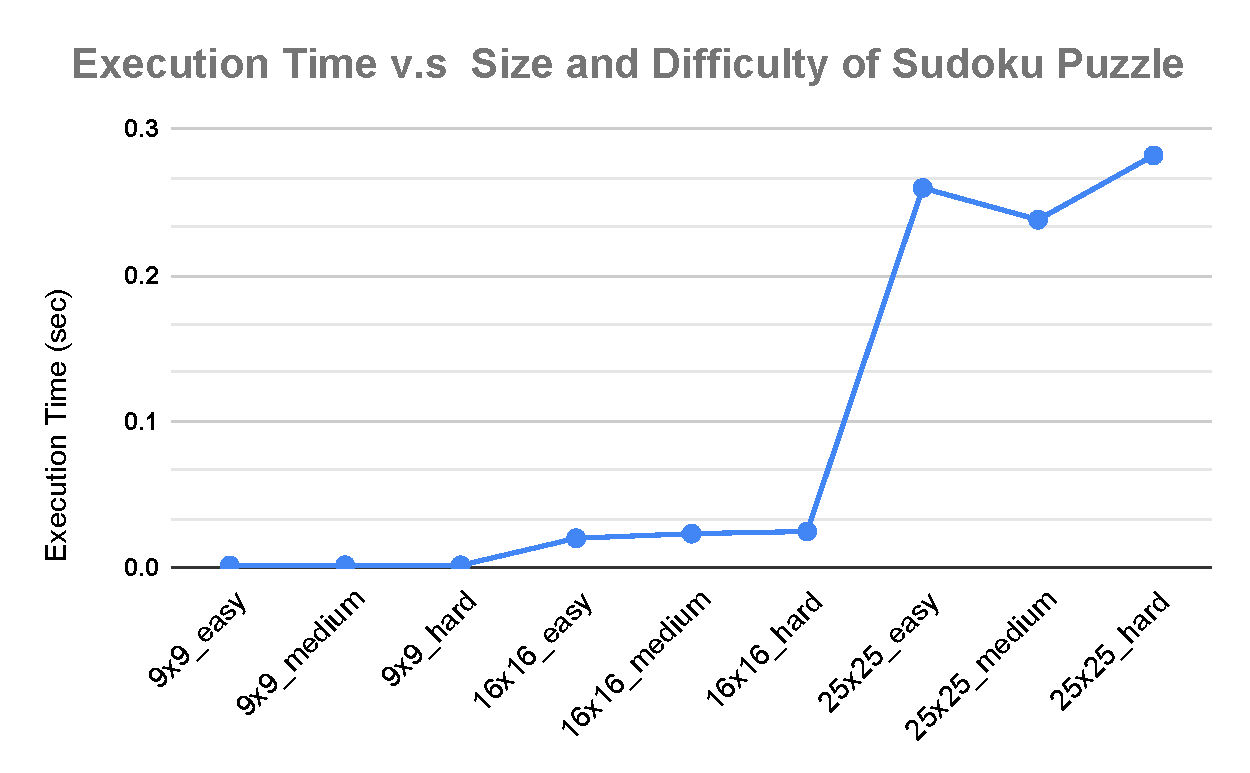
\includegraphics[width=0.7\linewidth]{sequential_DLX}}
			\caption{}
			\label{fig:sequential-dlx}
		\end{figure}

	\subsection{Parallel DLX algorithm}
	The Dancing Links algorithm does not appear to be very parallelizable.
	At its core, it is similar to the depth-first search (DFS) solving algorithms (i.e., backtracking, brute force)
	and will face similar parallelization challenges.
	Therefore, in this implementation I simply put the \code{solve} function into a parallel region and
	modify the \code{selectColumnNodeHeuristic} function to start with satisfying a different constraint in each thread.
	As expected, the performance doesn't benefit from parallelization because the sequential version performs well enough already.


% \subsubsection{Forward Checking / Elimination}
% The Forward Checking algorithm consists in verifying, after each assignment of a value
% to a variable, all the constraints in which the variable appears. It helps reducing the
% domain of the free variables that appear in these constraints.
% For example, in Sudoku, each time a value is assigned to a variable, the value is
% removed from the domain of the free variables that are either in the same line, in the
% same column or in the same square as the assigned variable.

% preventing possible future conflicts is more reasonable than recovering from them.


\section{Future Work}
As I had lots of fun and quite enjoyed in this project, I plan to do the following as future work:
\begin{itemize}
	\item Implement different solving algorithms (e.g., Forward Checking, Simulated Annealing, Constraint Propagation, etc.) in C++.
	\item Build GUI using QT library.
	\item Write unit tests using common unit testing frameworks, e.g., Google Test.
	\item Develop a Sudoku App for Android or iOS.
\end{itemize}


\newpage %%%%%%%%%%%%%%%%%%%%%%%%%%%%%%%%%%%%%%%%
\nocite{*}   % even non-cited BibTeX-Entries will be shown
\printbibliography[heading=bibintoc]


\end{document}